\chapter{Literature Review}
% \label{ch:relatedwork}
Over the past few years, Internet of Things or IoT, has had a significant impact in our lives.
It plays an important role whether it is a smartphone or a smarthome environment or just something 
as handy as a smartwatch. Different types of data is collected and exchanged among interconnected 
sensors/devices through modern communication network infrastructure connected by million of 
IoT nodes \cite{8123913,7598173,7879243,6774858,10.1145/2872332}. This direction of computing 
has already overtaken the traditional methods based on stationary computing \cite{8058399}. 
As a paradigm, IoT expresses that most physical devices, such as smart phones, smart watches and 
other embedded devices are interconnected with each other. These devices communicate with data 
centers and exchange information \textemdash all while adhering to their routine tasks \cite{7879243}. \\
Following various popular technologies these days, such as smart homes, smart grid and smart healthcare, 
IoT has become one of the essential components of people's home and workplace existence. It will 
continue to impact the daily life of people and its not just limited to technology. IoT has been reported 
to be one of the most important technologies that will impact US interests in 2025 \cite{7879243}. 
The number of interconnected physical devices has already transcended the human population for a couple 
years now. In 2012, there were 9 billion interconnected physical devices \cite{8058399}. This rapid increase 
in the number of mobile devices suggested that conventional centralized cloud computing would struggle 
to satisfy the Quality of Service (QoS) for many applications. However, with the introduction of 5G 
technology, edge computing becomes a viable and key solution to solve this issue \cite{7568592,7414384,6568922}. 
The edge computing platform allows edge nodes to respond to service demands which results in reduced 
bandwidth consumption and network latency. Figure \ref{fig:edgearch} shows a basic edge computing architecture. \\ 
\begin{figure}
    \begin{center}
        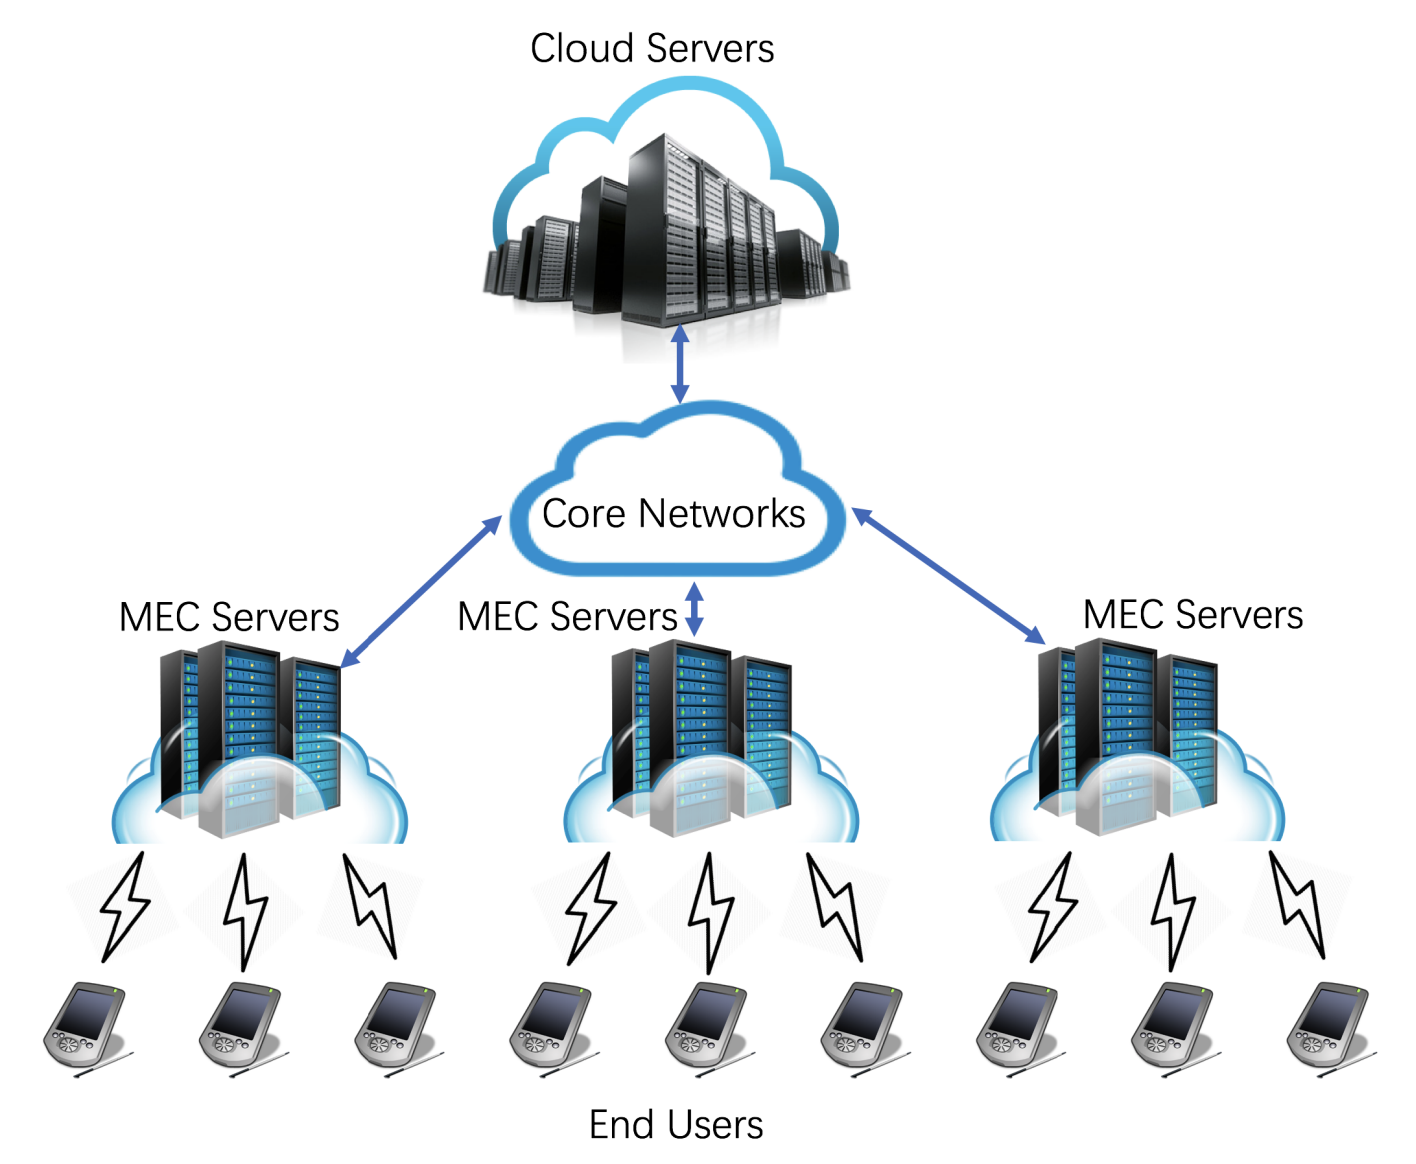
\includegraphics[scale=0.35]{Figs/edge_arch.png}    
    \end{center}
    \caption{The basic edge computing architecture}
    \label{fig:edgearch}
\end{figure}

Edge computing based IoT helps solve some critical issues and improves performance. Not to mention, IoT and 
edge computing share some characteristics which is further clarified by figure \ref{fig:edgeiot}. 
\begin{figure}
    \begin{center}
        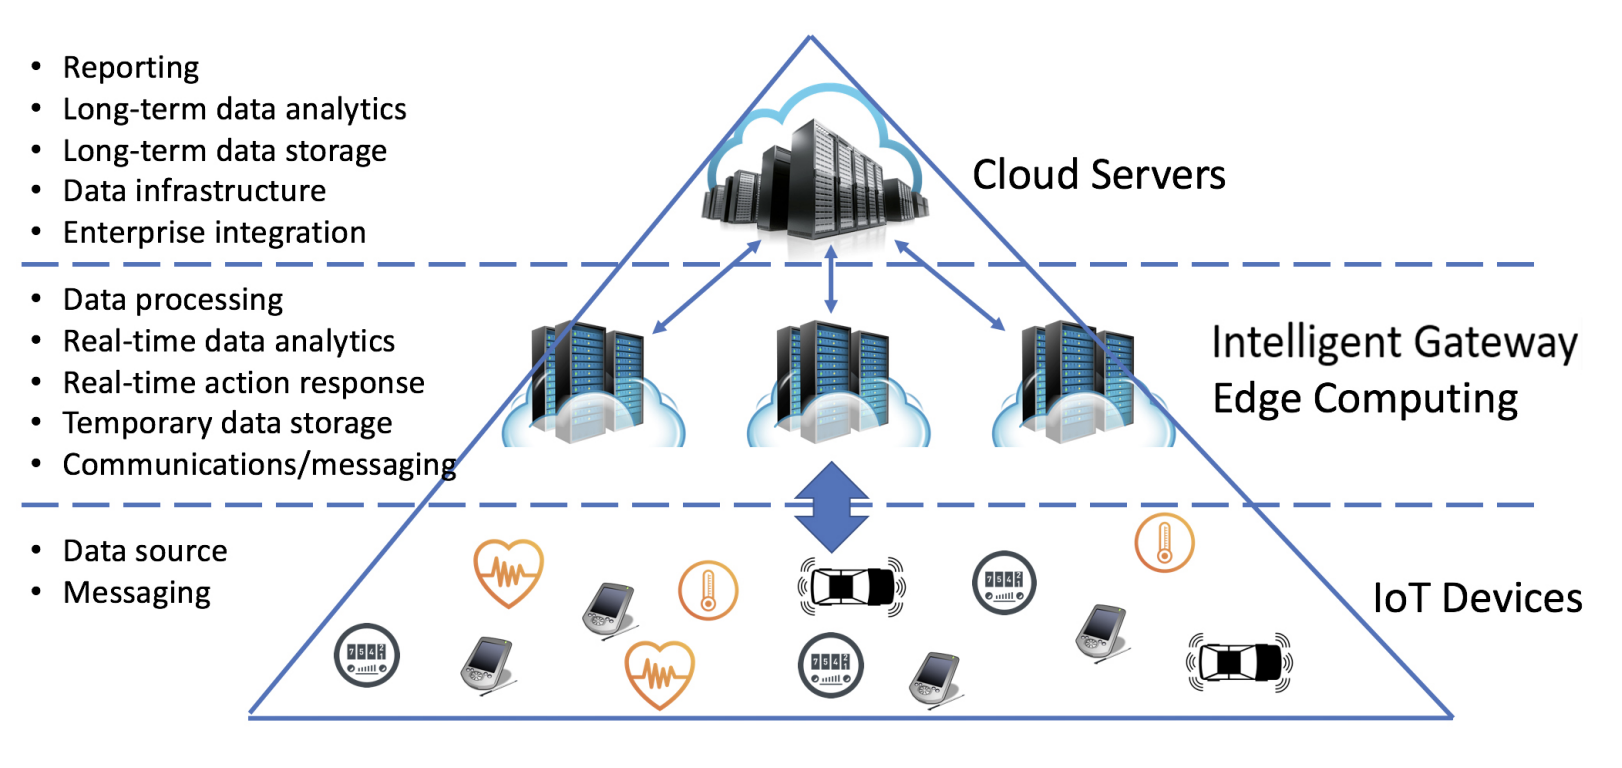
\includegraphics[scale=0.35]{Figs/edge_iot.png}    
    \end{center}
    \caption{Edge computing based IoT architecture}
    \label{fig:edgeiot}
\end{figure}

It further illustrates that IoT devices are end users for edge computing and IoT can benefit from both 
cloud and edge computing. The latter helps with faster response times and provides a tolerable computational 
capacity and storage space. Nowadays, the physical end user devices such as smart phones are considered 
edge devices. They may have an exclusively local component of an application but most generally, some sort of 
data is communicated with the cloud server, with or without the help of a gateway device. \\
One of the restricting factors among IoT edge devices is limited battery life (among limited storage and other things). 
